%% ODER: format ==         = "\mathrel{==}"
%% ODER: format /=         = "\neq "
%
%
\makeatletter
\@ifundefined{lhs2tex.lhs2tex.sty.read}%
  {\@namedef{lhs2tex.lhs2tex.sty.read}{}%
   \newcommand\SkipToFmtEnd{}%
   \newcommand\EndFmtInput{}%
   \long\def\SkipToFmtEnd#1\EndFmtInput{}%
  }\SkipToFmtEnd

\newcommand\ReadOnlyOnce[1]{\@ifundefined{#1}{\@namedef{#1}{}}\SkipToFmtEnd}
\usepackage{amstext}
\usepackage{amssymb}
\usepackage{stmaryrd}
\DeclareFontFamily{OT1}{cmtex}{}
\DeclareFontShape{OT1}{cmtex}{m}{n}
  {<5><6><7><8>cmtex8
   <9>cmtex9
   <10><10.95><12><14.4><17.28><20.74><24.88>cmtex10}{}
\DeclareFontShape{OT1}{cmtex}{m}{it}
  {<-> ssub * cmtt/m/it}{}
\newcommand{\texfamily}{\fontfamily{cmtex}\selectfont}
\DeclareFontShape{OT1}{cmtt}{bx}{n}
  {<5><6><7><8>cmtt8
   <9>cmbtt9
   <10><10.95><12><14.4><17.28><20.74><24.88>cmbtt10}{}
\DeclareFontShape{OT1}{cmtex}{bx}{n}
  {<-> ssub * cmtt/bx/n}{}
\newcommand{\tex}[1]{\text{\texfamily#1}}	% NEU

\newcommand{\Sp}{\hskip.33334em\relax}


\newcommand{\Conid}[1]{\mathit{#1}}
\newcommand{\Varid}[1]{\mathit{#1}}
\newcommand{\anonymous}{\kern0.06em \vbox{\hrule\@width.5em}}
\newcommand{\plus}{\mathbin{+\!\!\!+}}
\newcommand{\bind}{\mathbin{>\!\!\!>\mkern-6.7mu=}}
\newcommand{\rbind}{\mathbin{=\mkern-6.7mu<\!\!\!<}}% suggested by Neil Mitchell
\newcommand{\sequ}{\mathbin{>\!\!\!>}}
\renewcommand{\leq}{\leqslant}
\renewcommand{\geq}{\geqslant}
\usepackage{polytable}

%mathindent has to be defined
\@ifundefined{mathindent}%
  {\newdimen\mathindent\mathindent\leftmargini}%
  {}%

\def\resethooks{%
  \global\let\SaveRestoreHook\empty
  \global\let\ColumnHook\empty}
\newcommand*{\savecolumns}[1][default]%
  {\g@addto@macro\SaveRestoreHook{\savecolumns[#1]}}
\newcommand*{\restorecolumns}[1][default]%
  {\g@addto@macro\SaveRestoreHook{\restorecolumns[#1]}}
\newcommand*{\aligncolumn}[2]%
  {\g@addto@macro\ColumnHook{\column{#1}{#2}}}

\resethooks

\newcommand{\onelinecommentchars}{\quad-{}- }
\newcommand{\commentbeginchars}{\enskip\{-}
\newcommand{\commentendchars}{-\}\enskip}

\newcommand{\visiblecomments}{%
  \let\onelinecomment=\onelinecommentchars
  \let\commentbegin=\commentbeginchars
  \let\commentend=\commentendchars}

\newcommand{\invisiblecomments}{%
  \let\onelinecomment=\empty
  \let\commentbegin=\empty
  \let\commentend=\empty}

\visiblecomments

\newlength{\blanklineskip}
\setlength{\blanklineskip}{0.66084ex}

\newcommand{\hsindent}[1]{\quad}% default is fixed indentation
\let\hspre\empty
\let\hspost\empty
\newcommand{\NB}{\textbf{NB}}
\newcommand{\Todo}[1]{$\langle$\textbf{To do:}~#1$\rangle$}

\EndFmtInput
\makeatother
%
%
%
% First, let's redefine the forall, and the dot.
%
%
% This is made in such a way that after a forall, the next
% dot will be printed as a period, otherwise the formatting
% of `comp_` is used. By redefining `comp_`, as suitable
% composition operator can be chosen. Similarly, period_
% is used for the period.
%
\ReadOnlyOnce{forall.fmt}%
\makeatletter

% The HaskellResetHook is a list to which things can
% be added that reset the Haskell state to the beginning.
% This is to recover from states where the hacked intelligence
% is not sufficient.

\let\HaskellResetHook\empty
\newcommand*{\AtHaskellReset}[1]{%
  \g@addto@macro\HaskellResetHook{#1}}
\newcommand*{\HaskellReset}{\HaskellResetHook}

\global\let\hsforallread\empty

\newcommand\hsforall{\global\let\hsdot=\hsperiodonce}
\newcommand*\hsperiodonce[2]{#2\global\let\hsdot=\hscompose}
\newcommand*\hscompose[2]{#1}

\AtHaskellReset{\global\let\hsdot=\hscompose}

% In the beginning, we should reset Haskell once.
\HaskellReset

\makeatother
\EndFmtInput
%
%
%
%
%
% This package provides two environments suitable to take the place
% of hscode, called "plainhscode" and "arrayhscode". 
%
% The plain environment surrounds each code block by vertical space,
% and it uses \abovedisplayskip and \belowdisplayskip to get spacing
% similar to formulas. Note that if these dimensions are changed,
% the spacing around displayed math formulas changes as well.
% All code is indented using \leftskip.
%
% Changed 19.08.2004 to reflect changes in colorcode. Should work with
% CodeGroup.sty.
%
\ReadOnlyOnce{polycode.fmt}%
\makeatletter

\newcommand{\hsnewpar}[1]%
  {{\parskip=0pt\parindent=0pt\par\vskip #1\noindent}}

% can be used, for instance, to redefine the code size, by setting the
% command to \small or something alike
\newcommand{\hscodestyle}{}

% The command \sethscode can be used to switch the code formatting
% behaviour by mapping the hscode environment in the subst directive
% to a new LaTeX environment.

\newcommand{\sethscode}[1]%
  {\expandafter\let\expandafter\hscode\csname #1\endcsname
   \expandafter\let\expandafter\endhscode\csname end#1\endcsname}

% "compatibility" mode restores the non-polycode.fmt layout.

\newenvironment{compathscode}%
  {\par\noindent
   \advance\leftskip\mathindent
   \hscodestyle
   \let\\=\@normalcr
   \let\hspre\(\let\hspost\)%
   \pboxed}%
  {\endpboxed\)%
   \par\noindent
   \ignorespacesafterend}

\newcommand{\compaths}{\sethscode{compathscode}}

% "plain" mode is the proposed default.
% It should now work with \centering.
% This required some changes. The old version
% is still available for reference as oldplainhscode.

\newenvironment{plainhscode}%
  {\hsnewpar\abovedisplayskip
   \advance\leftskip\mathindent
   \hscodestyle
   \let\hspre\(\let\hspost\)%
   \pboxed}%
  {\endpboxed%
   \hsnewpar\belowdisplayskip
   \ignorespacesafterend}

\newenvironment{oldplainhscode}%
  {\hsnewpar\abovedisplayskip
   \advance\leftskip\mathindent
   \hscodestyle
   \let\\=\@normalcr
   \(\pboxed}%
  {\endpboxed\)%
   \hsnewpar\belowdisplayskip
   \ignorespacesafterend}

% Here, we make plainhscode the default environment.

\newcommand{\plainhs}{\sethscode{plainhscode}}
\newcommand{\oldplainhs}{\sethscode{oldplainhscode}}
\plainhs

% The arrayhscode is like plain, but makes use of polytable's
% parray environment which disallows page breaks in code blocks.

\newenvironment{arrayhscode}%
  {\hsnewpar\abovedisplayskip
   \advance\leftskip\mathindent
   \hscodestyle
   \let\\=\@normalcr
   \(\parray}%
  {\endparray\)%
   \hsnewpar\belowdisplayskip
   \ignorespacesafterend}

\newcommand{\arrayhs}{\sethscode{arrayhscode}}

% The mathhscode environment also makes use of polytable's parray 
% environment. It is supposed to be used only inside math mode 
% (I used it to typeset the type rules in my thesis).

\newenvironment{mathhscode}%
  {\parray}{\endparray}

\newcommand{\mathhs}{\sethscode{mathhscode}}

% texths is similar to mathhs, but works in text mode.

\newenvironment{texthscode}%
  {\(\parray}{\endparray\)}

\newcommand{\texths}{\sethscode{texthscode}}

% The framed environment places code in a framed box.

\def\codeframewidth{\arrayrulewidth}
\RequirePackage{calc}

\newenvironment{framedhscode}%
  {\parskip=\abovedisplayskip\par\noindent
   \hscodestyle
   \arrayrulewidth=\codeframewidth
   \tabular{@{}|p{\linewidth-2\arraycolsep-2\arrayrulewidth-2pt}|@{}}%
   \hline\framedhslinecorrect\\{-1.5ex}%
   \let\endoflinesave=\\
   \let\\=\@normalcr
   \(\pboxed}%
  {\endpboxed\)%
   \framedhslinecorrect\endoflinesave{.5ex}\hline
   \endtabular
   \parskip=\belowdisplayskip\par\noindent
   \ignorespacesafterend}

\newcommand{\framedhslinecorrect}[2]%
  {#1[#2]}

\newcommand{\framedhs}{\sethscode{framedhscode}}

% The inlinehscode environment is an experimental environment
% that can be used to typeset displayed code inline.

\newenvironment{inlinehscode}%
  {\(\def\column##1##2{}%
   \let\>\undefined\let\<\undefined\let\\\undefined
   \newcommand\>[1][]{}\newcommand\<[1][]{}\newcommand\\[1][]{}%
   \def\fromto##1##2##3{##3}%
   \def\nextline{}}{\) }%

\newcommand{\inlinehs}{\sethscode{inlinehscode}}

% The joincode environment is a separate environment that
% can be used to surround and thereby connect multiple code
% blocks.

\newenvironment{joincode}%
  {\let\orighscode=\hscode
   \let\origendhscode=\endhscode
   \def\endhscode{\def\hscode{\endgroup\def\@currenvir{hscode}\\}\begingroup}
   %\let\SaveRestoreHook=\empty
   %\let\ColumnHook=\empty
   %\let\resethooks=\empty
   \orighscode\def\hscode{\endgroup\def\@currenvir{hscode}}}%
  {\origendhscode
   \global\let\hscode=\orighscode
   \global\let\endhscode=\origendhscode}%

\makeatother
\EndFmtInput
%

\section{Introduction}
\label{sec:intro}

Theorem provers are actively used to mechanically verify large-scale
formalizations of critical components, including programming language
meta-theory~\cite{poplmark}, compilers~\cite{leroy09cc}, large
mathematical proofs~\cite{gonthier13engineering} and operating system
kernels~\cite{klein10seL4}. Due to their scale and complexity, these
developments can be quite time consuming, often demanding multiple
man-years of effort.

It is reasonable to expect that variations can simply
extend and reuse the original development in order to leverage the
large investment of resources in these formalizations.
This is unfortunately often not the case, as even small extensions
can require significant additional effort.
Adding a new language feature to a programming language formalization or
compiler, for example, involves significant redesigns that
have a cross-cutting impact on nearly all definitions and proofs in the
formalization. This leads to a copy-paste-patch approach to reuse with
several modified copies of the original development, making it difficult to
compose new features and ultimately leading to a maintenance nightmare.
%is desirable to structure their design as modularly as possible to
%enable easy modification and reuse. To this end, proof assistants such
%as Coq and Agda have powerful modularity constructs including modules,
%type classes and expressive forms of dependent types. Unfortunately,
%these modularity constructs are designed to support the addition of
%new definitions and proofs. When extension cut across these modularity
%boundaries by requiring a modification to existing definitions, as
%when adding a new piece of syntax to the expressions of a language,
%users are forced to manually edit the development, leading to a
%cut-paste-patch approach to reuse.
Dissatisfied with this situation, several
researchers~\cite{poplmark,shao10certified,stampoulis10VeriML,gonthier13engineering}
have called for better ways to modularize mechanical formalizations.

This work extends the current state-of-the-art in modular
mechanizations by solving a well-known and long-standing open problem
with denotational semantics: type soundness proofs are notoriously
brittle with respect to the addition of new effects. This is an
important problem because effects are pervasive in programming
language formalizations: in addition to extensions to syntax and
semantics, new features usually introduce new effects to the
denotations. Without a more robust formulation of type soundness, the
addition of new effects requires cross-cutting changes to type
soundness theorem statements and proofs.

Initially the semantics themselves were also brittle with respect to
effects~\cite{mosses84sdt,lee1989realistic}, but
\emph{monads}~\cite{Moggi89a,Wadler92a} have been found to provide the
necessary robustness to denotations. Yet as far as we know, the brittleness 
of (denotational) type soundness proofs has remained an open problem since it was raised by Wright and
Felleisen~\cite{wright94syntactic} to motivate their own type-soundness
approach. The framework we present here, \emph{modular monadic meta-theory} (\Name), is
the first in 20 years to provide a substantial solution. Using \Name, we develop a
novel approach to proving type soundness for monadic denotational
semantics in a way that is modular in the set of effects used. Proofs for
individual features do not depend on effects they do not use and hence
are robust to extension.

%%For example, it would be reasonable to expect that
%%after verifying a C compiler, verifying a C compiler with some
%%extensions requires a proportionaly equal effort to verify the language
%%extensions.
%Unfortunately, this is often not the case. Existing formal developments are
%usually \emph{monolithic} and extensions involve significant redesigns that
%have a pervasive impact on nearly all definitions and proofs in the
%formalization.

% \begin{figure}
% \begin{center}
% 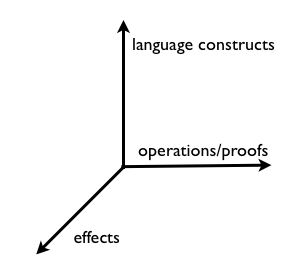
\includegraphics[scale=0.5]{src/modaxis.png}
% \end{center}
% \caption{Three dimensions of modularity.}
% \label{sec:axis}
% \vspace{-.5cm}
% \end{figure}

The solution builds on Meta-Theory \`{a} la Carte (MTC)~\cite{mtc}, a Coq
framework for the mechanization of formal programming language meta-theory that
supports modular extension of existing definitions. With MTC it is possible to
develop meta-theory which is modular in two dimensions: \emph{language features}
on the one hand and \emph{functions} and \emph{proofs} over these features on
the other hand. MTC adapts ideas from existing programming language
solutions~\cite{swierstra08dtc,oliveira09modular} to the \emph{expression
problem}~\cite{wadler98expression-problem} for functions and features, and adds
\emph{modular induction} for proofs.

\name adds a third modularity dimension to MTC: modular addition of new \emph{effects}. 
\name enables the separate definition of features with
effectful semantic functions and proofs over these functions, and reuse of
these features in formalizations of multiple languages.

To make denotations robust with respect to effects, \name uses the
established solution, \emph{monads}. In Coq, \emph{type
classes}~\cite{wadler89how-to} enable semantic function definitions
that are constrained, yet polymorphic in the monad. This allows the
inclusion of a feature in any language which supports a superset of
its effects. When a language is composed from different effectful
features, \emph{monad transformers}~\cite{liang95monad} are used to instantiate
the denotation's monad with all the effects required by the modular
components.

To solve the key challenge of modularizing and reusing theorems and proofs of 
type soundness, we split the classic type soundness theorems into three parts:
%%are highly challening because their traditional
%%formulations depend intimately
%%on the effects (such as state or exceptions) used by a language. As a
%%consequence, soundness statements over different sets of effects are
%%fundamentally incompatible and cannot be reused for supersets of
%%effects. \name overcomes this problem by splitting the problem into three
%%key theorems.
\begin{enumerate}
\item Reusable \emph{feature theorems} capture the essence
      of type soundness for an individual feature. 
      They depend only on that feature's syntax, typing relation, semantic function and the
      effects used therein. At the same time,
      they abstract over the syntax, semantics and effects of other features.
      This means that the addition of new features with other types of effects 
      \emph{does not affect} the existing feature theorem proofs. 

      To achieve the abstraction over other effects, a feature uses a constrained
      polymorphic monad. As a consequence, it only establishes the well-typing of the resulting
      denotations with respect to the effects declared in the constraints. 

\item Reusable \emph{effect theorems} fix the monad of denotations and consequently
      the set of effects. They take well-typing proofs of monadic denotations 
      expressed in terms of a constrained polymorphic monad and which mention only a subset of
      effects, and turn them into well-typings with respect to a fixed monad and all the effects it
      provides.
      
      Effect theorems reason fully at the level of denotations and
      abstract over the details of language features like syntax and semantic
      functions.

%       capture the overall interaction of
%       effects and evaluation for a particular combination of effects. Proofs
%       of this kind of theorem depend only on the set of effects used in
%       evaluation, and are orthogonal to features. Consequentely the same effect theorem
%       will work for any languages that use the particular combination of
%       effects captured by the theorem.



%%Proofs of this kind of theorem are independent
%%from any details of the features' semantic functions:
%%they only need to know that a feature preserves the reusable feature theorem.
\item Finally, \emph{language theorems} 
      establish type soundness for a particular language. 
      They require no more effort than to 
      instantiate the set of features and the set of effects (i.e., the monad), 
      thus tying together the respective feature and effect theorems into an overall proof.
\end{enumerate}
To establish the first two theorems, \name relies on modular induction and algebraic
laws about effects. As far as we know, it applies
the most comprehensive set of such laws to date, as
each effect utilized by a feature needs to
be backed up by laws and interactions between different
effects must also be governed by laws. These laws are crucial for
modular reasoning in the presence of effects.

% \BO{Expand and say something about case studies.}

\begin{comment}
An essential problem with existing development methodologies is that
they fail to deal with \emph{crosscutting concerns}. The problem is
not very different from problems which have been previously identified
in general software development.  As Tarr et al~\cite{f} argues most
programming languages tend to favor one form of decomposition, which
allows software to be modularized in certain way. Figure~\ref{sec:axis}
illustrates three different types of decomposition in which software
can be modularized. In the case of theorem provers like Coq, which can be viewed as functional
programming languages, the use of inductive datatypes allows
natural support for the modularization of \emph{operations} and \emph{proofs}.
However, as epitomized by the \emph{Expression Problem}~\cite{g}, if it is necessary
to extend the inductive datatypes with new cases then several
crosscutting changes are needed to update the operations and proofs.
Furthermore the introduction of effects in existing operations
requires pervasive changes to propagate effects in all
calling functions. In other words, while functional languages support
modularity naturally along the operations/proofs axis, they do not support
modularity well in the other two axis.


Previous work already provides three important ingredients towards
this goal: \emph{monads}~\cite{wadler}, \emph{modular
datatypes}~\cite{m} and \emph{modular induction}~\cite{e}. Monads are a
well-established way providing the semantics of languages with
effects; with the help of qualified types~\cite{j} and monad
transformers~\cite{k}, monads can be modularly composed. Modular
datatypes allow parts of a datatype and corresponding functions to be
defined separately and are helpful to localize particular features of
programming languages. Monads and modular datatypes have already
been shown to be an effective means to modularize

More recently it has been shown how to add
a modular form of induction on top of a variant of modular datatypes.
With modular induction it becomes possible to define

With monads and modular datatypes
semantic functions can be modularly defined for each language feature
without hard-wiring a particular set of effects or language
constructs~\cite{o}.

Previous work has already done significant progress towards
the development of modular techniques.

In previous work, we have proposed a solution for allowing modularity
in two dimensions simultaneously: operations/proofs and language constructs.
While for operations we were able, for the most part, to built on
existing solutions to the expression problem for mainstream languages,
dealing with proofs modularly required new techniques. In particular,
we had to develop new techniques which allowed us to express
\emph{inductive proofs} in a modular way. However, that work did
not provide a modular solution for effects. As a result, our meta-theory
framework was effectively limited to \emph{pure} languages.

In this work we provide a \emph{modular} solution for effects
that in combination with MTC allows the development of modular meta-theory
for languages with \emph{effects}. Much like our previous work,
dealing only with operations (not proofs) can, for the most part,
be done using existing techniques~\cite{j}. However, once again, the
key challenge lies in how to modularize theorems and proofs along the
three dimensions of modularity.
\end{comment}

\paragraph{}
In summary, the specific contributions of this work are:
\begin{itemize}

\item A reusable framework, \Name, for mechanized meta-theory of languages with effects.
This framework includes a mechanized library for monads, monad transformers and
corresponding algebraic laws in Coq. Besides several laws for
specific types of effects, the library also includes laws for
the interactions between different types of effects.

\item A new \emph{modular} proof method for type-soundness proofs of denotational semantics.

\item A case study of a family of fully mechanized languages, including
a mini-ML variant with errors and references. The case study comprises
28 languages, 8 different effect theorems and 5 features with their feature theorems.

\end{itemize}

\noindent\name is implemented in the Coq proof assistant and the code is available at
\url{http://www.cs.utexas.edu/~bendy/3MT}.
% Our implementation minimizes the
% programmer's burden for adding new features by automating the boilerplate with
% type classes and default tactics.
%%Moreover, the framework already provides modular
%%components for mini-ML as a starting point for new language formalizations.
% We also provide a complimentary Haskell
% implementation of the computational subset of code used in this paper.


%-------------------------------------------------------------------------------
\paragraph{Code and Notational Conventions}

While all the code underlying this paper has been developed in Coq,
the paper adopts a terser syntax for its many code fragments.  For the
computational parts, this syntax exactly coincides with Haskell
syntax, while it is an extrapolation of Haskell syntax style for
propositions and proof concepts. Following MTC, the Coq code requires the
impredicative-set option due to the use of Church encodings.

